\documentclass{article}
\usepackage{amsmath, amssymb}
\usepackage{tikz}
\usetikzlibrary{shapes.geometric, arrows}
\usepackage{graphicx}
\usepackage{hyperref}

\title{Technical Documentation: Modified Difference Boosting Neural Network (DBNN) for PyTorch}
\author{Ninan Sajeeth Philip\footnote{nsp@airis4d.com\\ Phone: +91 9496552479, +91 9497552476}\\ Artificial Intelligence Research and Intelligent Systems (airis4D))\\ Thelliyoor -689548\\ India}
\date{\today}

\begin{document}

\maketitle

\tableofcontents

\section{Introduction}
This document provides a detailed technical overview of the modified Difference Boosting Neural Network (DBNN) optimized for the PyTorch platform. The DBNN is a probabilistic neural network that leverages pairwise feature interactions to model complex data distributions. The modifications include GPU acceleration, adaptive learning, and improved handling of high-cardinality features.

\section{Architecture Overview}
The DBNN architecture consists of the following key components:
\begin{itemize}
    \item \textbf{Feature Pair Processing}: The model processes features in pairs, computing likelihoods for each pair.
    \item \textbf{Histogram and Gaussian Models}: The model supports both histogram-based and Gaussian-based likelihood computations.
    \item \textbf{Adaptive Learning}: The model adapts its learning rate and feature selection based on performance.
    \item \textbf{Invertible DBNN}: An optional invertible model for feature reconstruction.
\end{itemize}

\section{Mathematical Description}
\subsection{Likelihood Computation}
The likelihood of a feature pair $(x_i, x_j)$ given a class $c$ is computed as:
\[
P(x_i, x_j | c) = \sum_{k=1}^{K} w_{c,k} \cdot \text{PDF}(x_i, x_j | \theta_{c,k})
\]
where $w_{c,k}$ are the weights for class $c$ and feature pair $k$, and $\text{PDF}$ is the probability density function (either histogram-based or Gaussian).

\subsection{Posterior Probability}
The posterior probability of class $c$ given the feature vector $\mathbf{x}$ is:
\[
P(c | \mathbf{x}) = \frac{P(\mathbf{x} | c) \cdot P(c)}{\sum_{c'} P(\mathbf{x} | c') \cdot P(c')}
\]
where $P(c)$ is the prior probability of class $c$.

\subsection{Weight Update}
The weights are updated using the following rule:
\[
w_{c,k} \leftarrow w_{c,k} + \eta \cdot (1 - \frac{P(c | \mathbf{x})}{P(c' | \mathbf{x})})
\]
where $\eta$ is the learning rate, and $c'$ is the predicted class.

\section{Flowcharts}
\subsection{Training Process}
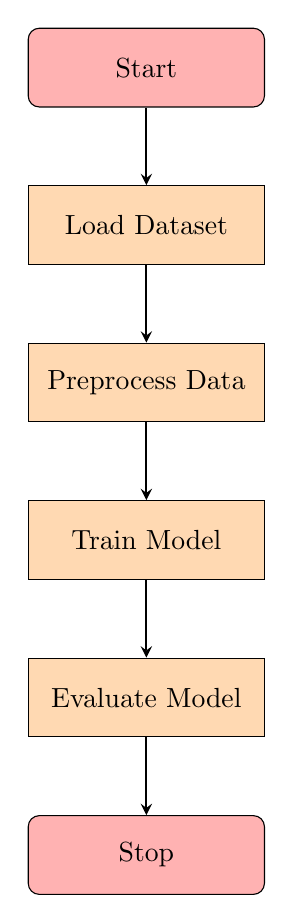
\begin{tikzpicture}[node distance=2cm]
    \tikzstyle{startstop} = [rectangle, rounded corners, minimum width=3cm, minimum height=1cm,text centered, draw=black, fill=red!30]
    \tikzstyle{process} = [rectangle, minimum width=3cm, minimum height=1cm, text centered, draw=black, fill=orange!30]
    \tikzstyle{decision} = [diamond, minimum width=3cm, minimum height=1cm, text centered, draw=black, fill=green!30]
    \tikzstyle{arrow} = [thick,->,>=stealth]

    \node (start) [startstop] {Start};
    \node (load) [process, below of=start] {Load Dataset};
    \node (preprocess) [process, below of=load] {Preprocess Data};
    \node (train) [process, below of=preprocess] {Train Model};
    \node (eval) [process, below of=train] {Evaluate Model};
    \node (stop) [startstop, below of=eval] {Stop};

    \draw [arrow] (start) -- (load);
    \draw [arrow] (load) -- (preprocess);
    \draw [arrow] (preprocess) -- (train);
    \draw [arrow] (train) -- (eval);
    \draw [arrow] (eval) -- (stop);
\end{tikzpicture}

\subsection{Adaptive Learning}
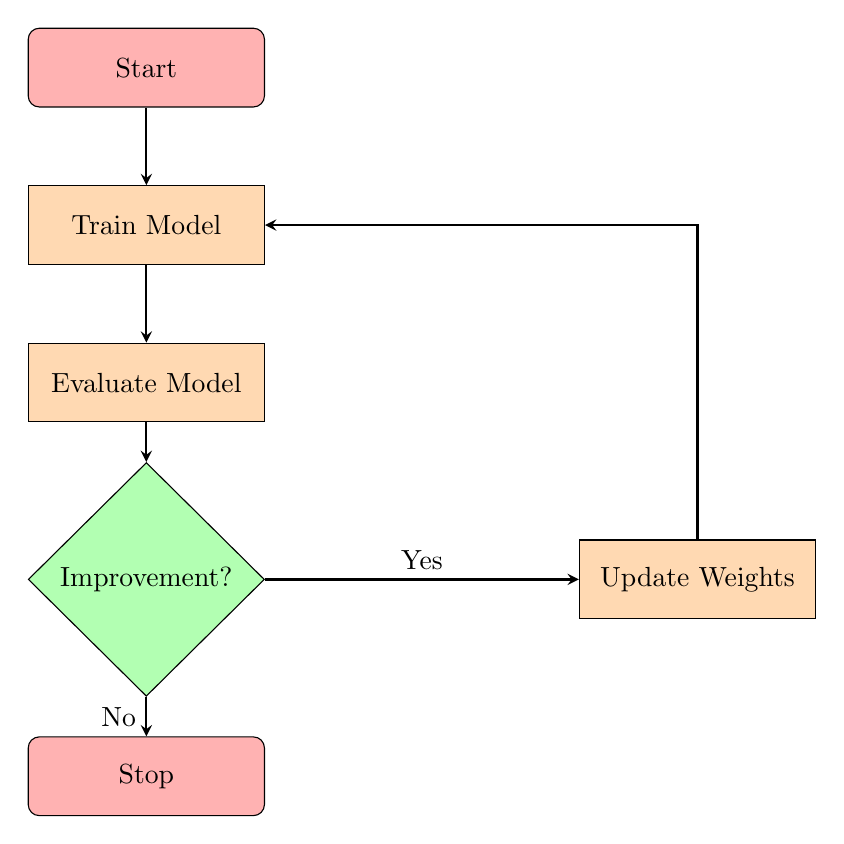
\begin{tikzpicture}[node distance=2cm]
    \tikzstyle{startstop} = [rectangle, rounded corners, minimum width=3cm, minimum height=1cm,text centered, draw=black, fill=red!30]
    \tikzstyle{process} = [rectangle, minimum width=3cm, minimum height=1cm, text centered, draw=black, fill=orange!30]
    \tikzstyle{decision} = [diamond, minimum width=3cm, minimum height=1cm, text centered, draw=black, fill=green!30]
    \tikzstyle{arrow} = [thick,->,>=stealth]

    \node (start) [startstop] {Start};
    \node (train) [process, below of=start] {Train Model};
    \node (eval) [process, below of=train] {Evaluate Model};
    \node (decide) [decision, below of=eval, yshift=-0.5cm] {Improvement?};
    \node (update) [process, right of=decide, xshift=5cm] {Update Weights};
    \node (stop) [startstop, below of=decide, yshift=-0.5cm] {Stop};

    \draw [arrow] (start) -- (train);
    \draw [arrow] (train) -- (eval);
    \draw [arrow] (eval) -- (decide);
    \draw [arrow] (decide) -- node[anchor=south] {Yes} (update);
    \draw [arrow] (update) |- (train);
    \draw [arrow] (decide) -- node[anchor=east] {No} (stop);
\end{tikzpicture}

\section{Features}
\subsection{GPU Acceleration}
The model is optimized for GPU acceleration using PyTorch's CUDA backend. This allows for faster computation of likelihoods and weight updates.

\subsection{Adaptive Learning}
The model includes an adaptive learning mechanism that adjusts the learning rate and feature selection based on performance. This helps in converging to a better solution faster.

\subsection{Invertible DBNN}
The model includes an optional invertible DBNN for feature reconstruction. This allows for the reconstruction of input features from the model's predictions.

\subsection{High-Cardinality Feature Handling}
The model includes improved handling of high-cardinality features by removing or rounding features with too many unique values.

\section{Conclusion}
The modified DBNN optimized for PyTorch provides a powerful tool for probabilistic modeling of complex data distributions. The inclusion of GPU acceleration, adaptive learning, and improved feature handling makes it suitable for a wide range of applications.

\end{document}
